% Options for packages loaded elsewhere
\PassOptionsToPackage{unicode}{hyperref}
\PassOptionsToPackage{hyphens}{url}
\PassOptionsToPackage{dvipsnames,svgnames,x11names}{xcolor}
%
\documentclass[
]{aft}

\usepackage{amsmath,amssymb}
\usepackage{iftex}
\ifPDFTeX
  \usepackage[T1]{fontenc}
  \usepackage[utf8]{inputenc}
  \usepackage{textcomp} % provide euro and other symbols
\else % if luatex or xetex
  \usepackage{unicode-math}
  \defaultfontfeatures{Scale=MatchLowercase}
  \defaultfontfeatures[\rmfamily]{Ligatures=TeX,Scale=1}
\fi
\usepackage{lmodern}
\ifPDFTeX\else  
    % xetex/luatex font selection
\fi
% Use upquote if available, for straight quotes in verbatim environments
\IfFileExists{upquote.sty}{\usepackage{upquote}}{}
\IfFileExists{microtype.sty}{% use microtype if available
  \usepackage[]{microtype}
  \UseMicrotypeSet[protrusion]{basicmath} % disable protrusion for tt fonts
}{}
\makeatletter
\@ifundefined{KOMAClassName}{% if non-KOMA class
  \IfFileExists{parskip.sty}{%
    \usepackage{parskip}
  }{% else
    \setlength{\parindent}{0pt}
    \setlength{\parskip}{6pt plus 2pt minus 1pt}}
}{% if KOMA class
  \KOMAoptions{parskip=half}}
\makeatother
\usepackage{xcolor}
\setlength{\emergencystretch}{3em} % prevent overfull lines
\setcounter{secnumdepth}{5}
% Make \paragraph and \subparagraph free-standing
\makeatletter
\ifx\paragraph\undefined\else
  \let\oldparagraph\paragraph
  \renewcommand{\paragraph}{
    \@ifstar
      \xxxParagraphStar
      \xxxParagraphNoStar
  }
  \newcommand{\xxxParagraphStar}[1]{\oldparagraph*{#1}\mbox{}}
  \newcommand{\xxxParagraphNoStar}[1]{\oldparagraph{#1}\mbox{}}
\fi
\ifx\subparagraph\undefined\else
  \let\oldsubparagraph\subparagraph
  \renewcommand{\subparagraph}{
    \@ifstar
      \xxxSubParagraphStar
      \xxxSubParagraphNoStar
  }
  \newcommand{\xxxSubParagraphStar}[1]{\oldsubparagraph*{#1}\mbox{}}
  \newcommand{\xxxSubParagraphNoStar}[1]{\oldsubparagraph{#1}\mbox{}}
\fi
\makeatother


\providecommand{\tightlist}{%
  \setlength{\itemsep}{0pt}\setlength{\parskip}{0pt}}\usepackage{longtable,booktabs,array}
\usepackage{calc} % for calculating minipage widths
% Correct order of tables after \paragraph or \subparagraph
\usepackage{etoolbox}
\makeatletter
\patchcmd\longtable{\par}{\if@noskipsec\mbox{}\fi\par}{}{}
\makeatother
% Allow footnotes in longtable head/foot
\IfFileExists{footnotehyper.sty}{\usepackage{footnotehyper}}{\usepackage{footnote}}
\makesavenoteenv{longtable}
\usepackage{graphicx}
\makeatletter
\def\maxwidth{\ifdim\Gin@nat@width>\linewidth\linewidth\else\Gin@nat@width\fi}
\def\maxheight{\ifdim\Gin@nat@height>\textheight\textheight\else\Gin@nat@height\fi}
\makeatother
% Scale images if necessary, so that they will not overflow the page
% margins by default, and it is still possible to overwrite the defaults
% using explicit options in \includegraphics[width, height, ...]{}
\setkeys{Gin}{width=\maxwidth,height=\maxheight,keepaspectratio}
% Set default figure placement to htbp
\makeatletter
\def\fps@figure{htbp}
\makeatother

\usepackage{booktabs}
\usepackage{longtable}
\usepackage{array}
\usepackage{multirow}
\usepackage{wrapfig}
\usepackage{float}
\usepackage{colortbl}
\usepackage{pdflscape}
\usepackage{tabu}
\usepackage{threeparttable}
\usepackage{threeparttablex}
\usepackage[normalem]{ulem}
\usepackage{makecell}
\usepackage{xcolor}
\usepackage{orcidlink}
\definecolor{mypink}{RGB}{219, 48, 122}
\makeatletter
\@ifpackageloaded{caption}{}{\usepackage{caption}}
\AtBeginDocument{%
\ifdefined\contentsname
  \renewcommand*\contentsname{Table of contents}
\else
  \newcommand\contentsname{Table of contents}
\fi
\ifdefined\listfigurename
  \renewcommand*\listfigurename{List of Figures}
\else
  \newcommand\listfigurename{List of Figures}
\fi
\ifdefined\listtablename
  \renewcommand*\listtablename{List of Tables}
\else
  \newcommand\listtablename{List of Tables}
\fi
\ifdefined\figurename
  \renewcommand*\figurename{Figure}
\else
  \newcommand\figurename{Figure}
\fi
\ifdefined\tablename
  \renewcommand*\tablename{Table}
\else
  \newcommand\tablename{Table}
\fi
}
\@ifpackageloaded{float}{}{\usepackage{float}}
\floatstyle{ruled}
\@ifundefined{c@chapter}{\newfloat{codelisting}{h}{lop}}{\newfloat{codelisting}{h}{lop}[chapter]}
\floatname{codelisting}{Listing}
\newcommand*\listoflistings{\listof{codelisting}{List of Listings}}
\makeatother
\makeatletter
\makeatother
\makeatletter
\@ifpackageloaded{caption}{}{\usepackage{caption}}
\@ifpackageloaded{subcaption}{}{\usepackage{subcaption}}
\makeatother

\ifLuaTeX
  \usepackage{selnolig}  % disable illegal ligatures
\fi
\usepackage[]{natbib}
\bibliographystyle{te}
\usepackage{bookmark}

\IfFileExists{xurl.sty}{\usepackage{xurl}}{} % add URL line breaks if available
\urlstyle{same} % disable monospaced font for URLs
\hypersetup{
  pdftitle={Modeling Longitudinal Binary Outcomes in a Small Matched-Pair Sample with Application to Cardiovascular Data: A Simulation Study},
  pdfauthor={Jinyu Luo; Chun-Po Steve Fan; Sudipta Saha; Aya Mitani},
  pdfkeywords={template, demo},
  colorlinks=true,
  linkcolor={blue},
  filecolor={Maroon},
  citecolor={Blue},
  urlcolor={red},
  pdfcreator={LaTeX via pandoc}}



\title{Modeling Longitudinal Binary Outcomes in a Small Matched-Pair
Sample with Application to Cardiovascular Data: A Simulation Study}
\author{
Jinyu Luo~\orcidlink{0009-0004-1101-7040}\\University of
Toronto\\\href{mailto:jinyu.luo@mail.utoronto.ca}{jinyu.luo@mail.utoronto.ca}\and 
Chun-Po Steve Fan~\orcidlink{0000-0002-6373-0532}\\University Health
Network\\\href{mailto:steve.fan@uhn.ca}{steve.fan@uhn.ca}\and 
Sudipta Saha\\University Health
Network\\\href{mailto:Sudipta.Saha@uhn.ca}{Sudipta.Saha@uhn.ca}\and 
Aya Mitani~\orcidlink{0000-0002-0373-5032}\\University of
Toronto\\\href{mailto:aya.mitani@utoronto.ca}{aya.mitani@utoronto.ca}}
\date{}
\begin{document}
\maketitle
\begin{abstract}
Background: This study aimed to address the challenge of modelling small
sample matched-pair longitudinal data in cardiovascular research. The
independent working correlation structure in Generalized Estimating
Equations (GEE), a robust method widely used to model endogenous
follow-up data, relies on large-sample theory. Prior research noted
significant constraints due to small sample sizes for continuous
outcomes. Objectives: We evaluated the validity of the working
independent correlation structure in GEE, specifically focusing on
binary outcomes, through a simulation study. Methods: Initially, real
hospital data were fitted, assuming a working exchangeable correlation
structure to estimate the true values for simulation parameters. The
simulations were designed to mimic the dropout process in the real-world
scenario where previous survival outcomes and associated covariates
influence the longitudinal outcomes. The simulated data involves
hospital cohorts with longitudinal outcomes across two exposure groups,
so cohorts were matched using propensity scores based on baseline
characteristics to eliminate potential confounding effects in
demographic and clinical characteristics. Due to the small sample size,
standard errors were adjusted by degrees of freedom to prevent
underestimation by the sandwich estimator. The simulated data was then
analyzed using three different correlation structures in GEE:
independent, exchangeable, and autoregressive (AR1). Results: The
independent working correlation structure in GEEs consistently provides
the highest coverage probabilities for true parameter coefficients after
adjusting for standard errors. Conclusion: Proper specification of the
correlation structure is important for the robust analysis of small
sample longitudinal data.
\end{abstract}


\section{Introduction}\label{sec-intro}

The generalized estimating equations (GEE) method is commonly used in
longitudinal studies where the response variable for each subject is
measured repeatedly over time \citep{LiangZeger1986}. It is an extension
of the quasi-likelihood method that models the marginal expectation of
the response, either discrete or binary, as a function of a set of
explanatory variables \citep{Agresti2nd}. Instead of assuming a
particular type of distribution for the outcome \(Y\), each marginal
mean is linked to a linear predictor and educated guess for the
variance-covariance structure, which accounts for the temporal
correlation among repeated measurements. Since there is no need to
specify the random effects for individual subjects or clusters, GEE
provides an average response in the population rather than
individual-specific effects.

Our motivation stems from the work which assessed the natural history of
the aortic root in patients with bicuspid versus tricuspid aortic valves
(BAVs vs.~TAVs) after replacement of the aortic valve and ascending
aorta at the Peter Munk Cardiac Center \citep{Hui2018}. The aorta is the
main artery that carries blood from the heart's left ventricle to the
rest of the human body. According to the 2014 ESC guidelines on
diagnosing and treating aortic diseases, aorta dilatation is a clinical
condition with aorta diameter greater than 40 mm, irrespective of body
surface area. It is commonly present in patients with BAV, a congenital
heart defect when the aortic valve has only two leaflets instead of
three and affects approximately 1-2\% of the general population
\citep{Wang2021}. Patients with aortic diameter exceeding 4.5 mm are
usually associated with ascending aortic events. Evidence showed that
the dilation of aortic root cannot be suppressed even after AVR
\citep{Bruce2003}. Still, other researchers found that the ascending
aorta dilatation rate was similar between the BAV and TAV post-surgery
\citep{KIM202053}.

Given that BAV is a congenital cardiac abnormality, conducting
randomized controlled trials is not feasible. Researchers often pair BAV
patients with TAV patients using propensity score matching (PSM) to
assess the natural history of aortic root size changes. PSM is critical
in this context as it balances observed covariates between BAV and TAV
groups, reducing confounding bias and enhancing the accuracy of
treatment effect estimates. This technique allows for valid comparisons
in observational studies, addressing selection bias and leading to more
reliable conclusions about the natural history of aortic root size
changes post-surgery. In practice, patients with and without exposure to
interest are matched on important confounding factors such as age, sex,
and calendar time and compared for the incidence of outcomes
\citep{Iwagami2022}. In such a scenario, two distinct correlations
exist: the correlation between units within the matched pair and the
correlation between the temporal observations on the same patient. The
study investigators collected participant-level demographics, health
outcomes, and each participant's follow-up imaging data after the
replacement of the aortic valve (AVR) and ascending aorta (RAA) from
January 1900 to December 2010. This cohort consists of 406 patients, 244
of whom had follow-up measurements. Among those with follow-up visits,
172 (70.5\%) patients had BAV, and the rest had TAV. Our primary outcome
is whether or not the aortic root dimensions exceeded a diameter of 45
mm after the surgery. Although the data include records of patients'
vitals, only the follow-up measurements of the aortic root size and
baseline covariates, including age, sex, and body surface area (BSA),
are included in this study.

The first consideration in GEE analysis is the potential issue of
covariate endogeneity. This concept describes the scenario when the
response at time \(t\) predicts the covariate value at times \(s > t\)
\citep{Diggle2002}. The issue arises because the abnormal aortic root
size is associated with a higher risk of death \citep{KITAGAWA2013258},
and the occurrence of death informs that there is no stochastic process
of the deformation. The interaction effect between response and
covariates is called \emph{feedback} \citep{Zeger1991}. It has been
shown that, based on the large-sample theory, using GEE with a working
independence correlation structure can provide unbiased estimation
\citep[@LiangZeger1986]{Diggle2002}. However, the sample sizes in
cardiovascular research are limited and mid-term follow-ups are
incomplete due to the rarity of disease in practice. The validity of GEE
with a working independence correlation structure remains unknown. The
second consideration is that GEE methods within the existing R package,
i.e., \texttt{geepack,} only account for the correlation between
repeated measurements within one subject but ignore the correlation
between matched pairs.

This report focuses on matched longitudinal binary data with covariate
endogeneity and informative dropouts. We aim to explore the validity of
GEE estimates for small sample matched-pair binary outcomes and compare
the estimation results with the two-stage quasi-least squares (QLS)
method \citep{Mitani2019}. In section 2, we described the issue with the
correlation structure and the construction of two-stage QLS method in
more detail. The simulation study design is presented in section 3. In
section 4, exploratory data analysis and model fitting results on the
motivational data and simulated data are presented. Finally, we conclude
this reports with a discussion in section 5.

\section{Methods}\label{methods}

Consider a longitudinal matched data set in which subjects are grouped
into pairs, and each subject contributes repeated observations of unique
aortic root diameter. Let \(Y_{ijk}\) be the binary outcome measurement
of the \(k^{th}\) visit on the \(j^{th}\) subject from the \(i^{th}\)
pair, where \(k = 1,...,t_{ij}, j = 1,2\) and \(i = 1,..., N\). Here,
\(t_{ij}\) is the total number of visit for the \(j^{th}\) subject from
the \(i^{th}\) pair. Let \(X_{ijk}\) be the \(p\times 1\) vector of
covariates for the outcome \(Y_{ijk}\) of the \(k^{th}\) visit of the
\(j^{th}\) subject from the \(i^{th}\) pair. In our case, \(X_{ijk}\)
includes BAV (exposure), \emph{time}, and the interaction between BAV
and \emph{time}. Because different patients may have different follow-up
intervals, we define \emph{time} as the number of visits.

Given that the outcome \(Y_{ijk}\) is binary, the marginal expectation
for the \(k^{th}\) visit on the \(j^{th}\) subject from the \(i^{th}\)
pair is \begin{equation}
\mu_{ijk} = E(Y_{ijk}|X_{ijk}). \label{eq:marginExpecatiton}
\end{equation} We use a logit link function to relate the marginal
expectation \(\mu_{ijk}\) to the linear predictor. The logit link
function is defined as: \[
\begin{aligned}
\text{logit}(\mu_{ijk}) &= \log(\frac{\mu_{ijk}}{1-\mu_{ijk}})= g(\mu_{ijk}) \\
&= \beta_0 + \beta_1 \times \text{BAV}_{ij} + \beta_2 \times \text{Visit}_{ijk}+\beta_3 (\text{BAV}_{ij}\times \text{Visit}_{ijk})\\
& = X_{ij}^T\boldsymbol{\beta}
\end{aligned}
\] where \(\boldsymbol{\beta} = (\beta_0, \beta_1, \beta_2, \beta_3)^T\)
is the set of regression coefficients to be estimated (Note: The
exposure variable, BAV, will not change with time, so its subscript only
varied for \(i\) and \(j\)). Then, the variance can be expressed as:
\begin{equation}
\text{Var}(Y_{ijk}) = \mu_{ijk}(1-\mu_{ijk}) = h(\mu_{ijk}) \label{eq:marginVariance}
\end{equation}

\subsection{Generalized estimating equations
(GEE)}\label{generalized-estimating-equations-gee}

Without a specific assumption about the likelihood function, generalized
estimating equations (GEE) accounts the covariance structure of the
repeated measures by specifying a working correlation matrix,
\(R(\alpha)\), which describes the correlation between repeated measures
on the same subject. This paper focuses on the following three working
correlations: \[
\underset{\text{(Independent)}}{\begin{bmatrix}
1 & 0 & \cdots & 0\\
0 & 1 & \cdots &  0\\
\vdots & \vdots & \ddots & \vdots\\
0 & 0 & \cdots & 1
\end{bmatrix}}
\quad
\underset{\text{(Exchangeable)}}{\begin{bmatrix}
1 & \alpha & \cdots & \alpha\\
\alpha & 1 & \cdots & \alpha\\
\vdots & \vdots & \ddots & \vdots\\
\alpha & \alpha & \cdots & 1
\end{bmatrix}}
\quad
\underset{\text{(AR1)}}{\begin{bmatrix}
1 & \alpha & \cdots & \alpha^{t_{ij} - 1}\\
\alpha & 1 & \cdots & \alpha^{t_{ij} - 2}\\
\vdots & \vdots & \ddots & \vdots\\
\alpha^{t_{ij} - 1} & \alpha^{t_{ij} - 2} & \cdots & 1
\end{bmatrix}}
\] . The independent working correlation assumes no correlation between
repeated measures. With a correlation coefficient \(\alpha\), the
exchangeable working correlation assumes that the correlation between
any pair of repeated measurements are constant at \(\alpha\), whereas
the autoregressive order one (AR1) working correlation structure assumes
correlation decreases exponentially with the time lag between measures.
GEE approach accounts for overdispersion or underdispersion by
correcting the variance using a dispersion parameter \[
\text{Var}(Y_{ijk})^* = \phi\text{Var}(Y_{ijk}) = \phi h(\mu_ijk)
\]

The marginal expectation, \(\mu_{ij}\) can be expressed as
\(\mu_{ij} = \left[g^{-1}(X_{ij1}^T \boldsymbol{\beta}), ..., g^{-1}(X_{ijt_{ij}}^T \boldsymbol{\beta})\right]^T\),
then we define \(A_{ij} = diag\{h(\mu_{ij1}),...h(\mu_{ijt_{ij}})\}\).
The working covariance matrix for subject \(j^{th}\) from the \(i^{th}\)
pair is \(\Sigma_i = A_i^{1/2}R(\alpha)A_i^{1/2}\). Let \(\phi\) be the
dispersion parameter, then \(\Sigma_i \phi\) is the covariance working
matrix. Since our outcome is binary, the dispersion parameter \(\phi\)
equals to 1.

The iterative process starts with initial guesses for the regression
coefficients \(\boldsymbol{\beta}^{(0)}\) and the correlation parameters
\(\alpha^{(0)}\). It is followed by the computation of initial marginal
expectation
\(\mu_{ijk}^{(0)} = g^{-1}(X_{ijk}^T \boldsymbol{\beta}^{(0)})\), where
\(g^{-1}\) is the inverse of the link function. Then, the iterative
process mainly consists of two steps: (1) update the working correlation
matrix using the sample data. (2) update the regression coefficients.

\subsubsection{Update the Working Correlation
Matrix}\label{update-the-working-correlation-matrix}

To update the working correlation matrix, we first compute the
residuals, \(r_{ijk}^{(m)} = Y_{ijk} - \mu_{ijk}^{(m)}\), based on the
current estimates of the marginal means for each observation. Then, we
estimate the correlation parameters using the residuals and construct
the working correlation matrix \(R_i^{(m)}(\alpha^{(m)})\) using the
updated correlation parameters.

\subsubsection{Update the Regression
Coefficients}\label{update-the-regression-coefficients}

For each subject, we compute the variance matrix using the current
estimates of the marginal means: \begin{equation}
\Sigma_i(\alpha) = A_i^{1/2}R(\alpha)A_i^{1/2} \label{eq:geeCovMat}
\end{equation} where \(A_i^{1/2}\) is a diagonal matrix with the
variances \(\mu_{ijk}^{(m)} (1-\mu_{ijk}^{(m)})\) on the diagonal. Then,
the score function and the information matrix can be calculated using
the current estimates \citep{Zeger1988}: \begin{align}
\boldsymbol{U}(\boldsymbol{\beta}) &= \sum_{i=1}^N D_i^T \Sigma_i^{-1}(\alpha) (Y_i - \mu_i) \label{eq:geeScoreEqs}\\
I(\boldsymbol{\beta}) &= \sum_{i=1}^N D_i^T\Sigma_i^{-1}(\alpha)D_i \label{eq:geeInfoMat}
\end{align} where
\(D_i = \frac{\partial\mu_i}{\partial \boldsymbol{\beta}}\). The new set
of regression coefficients are obtained by solving the score function,
which are then used to calculate the new marginal means.

The final estimates of the regression coefficients
\(\boldsymbol{\beta}\) can be obtained by repeat the above process until
convergence is achieved \citep{Liang1986}. This iterative process
ensures that the correlation structure and the regression coefficients
are appropriately updated using the sample data, resulting in consistent
and efficient parameter estimates in the presence of correlated repeated
measures.

However, it has been shown that the sandwich estimator tends to
underestimate standard errors (SEs) when the size sample data is small
\citep{Mitani2019}. To overcome this issue, we can adjust the sandwich
estimator by degrees of freedom \citep{dfcorrect}: \begin{equation}
\Sigma_{DF} = (\frac{N}{N-p})\Sigma \label{eq:geeSigmaDF}
\end{equation} where \(N\) represents the number of patients, \(p\) is
the number of regression parameters.

\subsection{Quasi-least squares (QLS)}\label{quasi-least-squares-qls}

Quasi-least squares (QLS) is a two-stage approach for estimating the
correlation parameters in the framework of generalized estimating
equations (GEE). The method involves estimating the regression
parameters and the correlation structure in two distinct stages.
Proposed by \citet{qls}, the two-stage QLS method assumes that the
covariance matrix are functions of the regression parameters and
independent of the dispersion parameter \(\phi\). Additionally, the
off-diagonal elements are functions of some unknown nuisance parameters.
The first stage mainly aims to estimate the regression parameters by
minimizing the score function, which is consistent with the GEE
approach. The difference is that the QLS method solves an unbiased
estimating equation for \(\alpha\), whereas the GEE method implements
moment estimates of the correlation parameters \citep{qlspack}. The
second stage refines the estimates of the correlation parameters based
on the residuals from the first stage and updates the working
correlation matrix. By iterating between these two stages, the two-stage
QLS approach ensures robust and efficient estimates of the regression
parameters while appropriately accounting for the correlation within the
data.

In our context, the goal is to fit a logistic regression model to
describe the relationship between the covariates and the binary outcome
of whether the aortic root diameter exceeds a specified threshold:
\begin{equation}
\text{logit}[\text{Pr}(Y_{ijk} = 1)] = X_{ijk}^T \boldsymbol{\beta} = \mu_{ijk} \label{eq:qlsMarginExpectation}
\end{equation} where \(Y_{ijk}\) is the binary outcome for the
\(k^{th}\) visit of the \(j^{th}\) subject from the \(i^{th}\) pair,
\(X_{ijk}\) is the vector of covariates, and \(\boldsymbol{\beta}\) is
the vector of regression coefficients. The dependence between the binary
response will be incorporated in the working correlation matrix.

Using matrix notation, we group each of the response vectors of the
\(j^{th}\) unit from the \(i^{th}\) pair as
\(\boldsymbol{Y}^T_{ij} = (\boldsymbol{Y}^T_{ij1}, ..., \boldsymbol{Y}^T_{ijt_{ij}})\).
Similarly, let \(\boldsymbol{u}_{ij} = E(\boldsymbol{Y}_{ij})\), where
\(\boldsymbol{u}^T_{ij} = (\boldsymbol{u}^T_{ij1}, ..., \boldsymbol{u}^T_{ijt_{ij}})\)
and
\(\boldsymbol{u}^T_{ijk} = (\boldsymbol{u}^T_{ijk0}, \boldsymbol{u}^T_{ijk1})\)
representing the outcome for TAV and BAV, respectively. For each pair
\(i\), define the complete data matrix for the \(j^{th}\) subject as \[
X_{ij} = (\boldsymbol{1}_{t_{ij}} \otimes 1, X_{0ij} \otimes 1)
\] where \(X_{0ij}\) indicates that this matrix contains the baseline
covariates for the \(j^{th}\) subject in the \(i^{th}\) pair and
\(\otimes\) represents the Kronecker product \citep{parson2006}. Define
\(A_{ij}\) and \(\Sigma_{ij}\) in the same way as the GEE approach, and
let
\(\boldsymbol{Z}_{ij}^T = (\boldsymbol{Y}_{ij} - \mu_{ij})^T A_{ij}^{1/2}\).
Then, the generalized sum of squares is defined as \citep{Mitani2019}:
\begin{equation}
Q_W(\alpha, \beta) = \sum_{i=1}^N\frac{1}{2}\left(\frac{1}{t_{i1}}Z^T_{i1}\Sigma_{i1}^{-1} Z_{i1} + \frac{1}{t_{i2}}Z^T_{i2}\Sigma_{i2}^{-1} Z_{i2}\right) = 0 \label{eq:qlsGSS}
\end{equation}

\subsubsection{\texorpdfstring{Specification of
\(\Sigma_{ij}\)}{Specification of \textbackslash Sigma\_\{ij\}}}\label{specification-of-sigma_ij}

The working correlation is specified using the approach proposed by
\citet{parson2006}. Let \(\Sigma_i(\Gamma)\) be the working correlation
matrix of the outcome vector for the \(i^{th}\) pair with the working
correlation parameter \(\Gamma^T = (\tau^T, \alpha^T)\) where \(\tau\)
represents the correlation within matched pairs and \(\alpha\) denotes
the correlation between longitudinal measurements. The working
correlation matrix can be specified as \begin{equation}
\Sigma_i = C_i(\tau) \otimes R_i(\alpha) \label{eq:qlsCovMat}
\end{equation} where \[
C_i(\tau) = 
\begin{bmatrix}
1 & \tau \\
\tau & 1
\end{bmatrix}; 
\quad 
R_i(\alpha) = 
\begin{bmatrix}
1 & \alpha & \alpha^2 & \alpha^3\\
\alpha & 1 & \alpha & \alpha^2\\
\alpha^2 & \alpha & 1 & \alpha\\
\alpha^3 & \alpha^2 & \alpha & 1
\end{bmatrix}
\] assuming the total number of visit \(t_{ij} = 4\) and the working
correlation structure is AR1.

\subsubsection{\texorpdfstring{Estimation of \(\beta\) and
\(\alpha\)}{Estimation of \textbackslash beta and \textbackslash alpha}}\label{estimation-of-beta-and-alpha}

Taking the partial derivative of \(Q_W(\alpha, \boldsymbol{\beta})\)
\eqref{eq:qlsGSS} with respect to \(\boldsymbol{\beta}\) and setting it
equal to 0, the score function is \begin{equation}
S(\boldsymbol{\beta}) = \sum_{i=1}^N \frac{1}{2} \left(\frac{1}{t_{i1}}\boldsymbol{D}_{i1}^T \boldsymbol{W}_{i1}^{-1}(\boldsymbol{Y}_{i1} - \boldsymbol{\mu}_{i1}) + \frac{1}{t_{i2}}\boldsymbol{D}_{i2}^T \boldsymbol{W}_{i2}^{-1}(\boldsymbol{Y}_{i2} - \boldsymbol{\mu}_{i2})\right) = 0  \label{eq:qlsScore}
\end{equation} where
\(\boldsymbol{D}_{ij} = \partial \boldsymbol{\mu}_{ij} / \partial \beta\)
and
\(\boldsymbol{W}_{ij} = A_{ij}^{1/2} Sigma_{ij}(\alpha) A_{ij}^{1/2}\).
With the correct specification of the working correlation
\(Sigma_{ij}\), we can interpret the marginalization as the binary
outcomes of aortic root diameter measurements over time for each subject
within a matched pair. This approach allows us to model the effects of
covariates while accounting for within-pair correlations and
longitudinal dependencies.

The estimation of \(\alpha\) involves two stages. The first stage
estimates \(\alpha\) by taking the partial derivative of
\(Q_W(\alpha, \beta)\) with respect to \(\alpha\) and setting it equal
to 0: \begin{equation}
\sum_{i=1}^N \frac{1}{2} \left(\frac{1}{t_{i1}}\boldsymbol{Z}_{i1}^T\frac{\partial \Sigma_{i1}^{-1}}{\partial \alpha}\boldsymbol{Z}_{i1} + \frac{1}{t_{i2}}\boldsymbol{Z}_{i2}^T \frac{\partial \Sigma_{i2}^{-1}}{\partial \alpha}\boldsymbol{Z}_{i2}\right) = 0  \label{eq:stage1alpha}
\end{equation} Since the stage one estimator for \(\alpha\) is
asymptotically biased \citep{CHAGANTY1999145}, a consistent estimator
can be obtained through the second stage by solving the following
equation for \(\alpha\): \begin{equation}
\sum_{i=1}^N \frac{1}{2} \left[\frac{1}{t_{i1}}\text{trace}\left(\frac{\partial \Sigma_{i1}^{-1} (\hat{\alpha}_0)}{\partial \hat{\alpha}_0}\Sigma_{i1}(\alpha)+\frac{\partial \Sigma_{i2}^{-1} (\hat{\alpha}_0)}{\partial \hat{\alpha}_0}\Sigma_{i2}(\alpha)\right)\right] \label{eq:stage2alpha}
\end{equation} where \(\hat{\alpha}_0\) is the solution to equation
\eqref{eq:stage1alpha}. The estimator for \(\boldsymbol{\beta}\) and
\(\alpha\) are obtained by choosing a starting value for
\(\boldsymbol{\beta}\) from fitting a GLM assuming independence between
observations and iterating through equations \eqref{eq:qlsScore},
\eqref{eq:stage1alpha}, and \eqref{eq:stage2alpha}.

\subsection{AR1 working correlation
structure}\label{ar1-working-correlation-structure}

Given that all the subjects from the motivational study underwent the
aortic root replacement surgery, it is reasonable to believe that the
correlation of longitudinal measurements is decreasing as time passes.
Therefore, AR1 is assumed to be the true working correlation structure.
Then, a closed-form solution for equation \eqref{eq:stage1alpha} can be
obtained by solving the following formula: \begin{equation}
\hat{\alpha}_0 = \frac{F_a + \sqrt{(F_1+F_b)(F_a-F_b)}}{F_b} \label{eq:ar1alpha1}
\end{equation} where \[
F_a = \sum_{i=1}^N \frac{1}{2} \sum_{j=1}^2 \frac{1}{t_{ij}}\left[\sum_{k=1}^{t_{ij}} Z_{ijk}^T C_i^{-1} Z_{ijk} + \sum_{k=1}^{t_{ij}-1}Z_{ijk}^T C_i^{-1} Z_{ijk}\right]
\] and
\(F_b = 2\sum_{i=1}^N \frac{1}{2}\sum_{j=1}^2\frac{1}{t_{ij}}\sum_{k=1}^{t_{ij}-1} Z_{ijk}^T C_i^{-1} Z_{ijk+1}\).
The stage two estimator for \(\alpha\) can be obtained by solving the
equation \eqref{eq:stage1alpha} \citep{Mitani2019}: \begin{equation}
\hat{\alpha} = \frac{2\hat{\alpha}_0}{1+\hat{\alpha}_0^2} \label{eq:ar1alpha2}
\end{equation}. Detailes of the derivations for equation
\eqref{eq:ar1alpha1} and \eqref{eq:ar1alpha2} are shown in the Appendix.

\subsection{Modeling Motivational
Data}\label{modeling-motivational-data}

To model the motivational data, we first selected all patients who had
at least one follow-up visit with baseline measurement being taken at
the day of operation. Then, a binary outcome was created by setting it
to 1 if the current root size measurement is over 45 mm or the growth
from the previous measure is over 5 mm, and 0 otherwise. A maximal of 6
records (including the baseline) for each patient were kept for further
analysis. Then, assuming that dropouts follows Weibull distribution, 5
survival models were fitted from visit 2 to 6. The fitting coefficients
were extracted for simulation. Next, a logistic regression model is
fitted on the data which included the baseline measurements so that we
can pair BAV patients with TAV patients using the \texttt{pairmatch}
function from the R package \texttt{optmatch} \citep{optmatch}. Then, we
applied the function \texttt{geeglm} from the R package \texttt{geepack}
on the matched data set to produce the estimation results using
independence, exchangeable, and AR1 working correlation structures.
Finally, customized functions for implementing QLS are applied on the
matched data.

\section{Simulation Study}\label{simulation-study}

\subsection{Full Data Simulation}\label{full-data-simulation}

The simulation process for generating one set of cohort data involves
several steps to model both covariates and binary outcomes for each
patient. For each patient, we first simulated baseline covariates,
including age, sex, and body surface area (BSA), by assuming a normal
distribution for continuous data and a binomial distribution for binary
data. To calculate the probability of having BAV, we used a logistic
regression model of the form: \[
\text{Pr}(\text{BAV} = 1 | \text{Age, Sex, BSA}) = \frac{\exp(\gamma_0 + \gamma_1 \cdot \text{Age} + \gamma_2 \cdot \text{Sex} + \gamma_3 \text{BSA})}{1+\exp(\gamma_0 + \gamma_1 \cdot \text{Age} + \gamma_2 \cdot \text{Sex} + \gamma_3 \text{BSA})}
\] where \(\gamma_0 = -0.407, \gamma_1 = -0.071, \gamma_2 = 1.231\), and
\(\gamma_3 = 3.038\). This probability is then used to generate the
exposure variable, BAV, under binomial distribution. To simulate
longitudinal matched data with binary outcomes, the marginal probability
of having positive outcome is obtained by using another logistic
regression model that includes BAV, visit times, and their interaction:
\[
\text{Pr}(Y = 1 | \text{BAV, Visit, BAV} \times \text{Visit}) = \frac{\exp(\beta_0 + \beta_1 \cdot \text{BAV} + \beta_2 \cdot \text{Visit} + \beta_3 \cdot \text{BAV}\cdot \text{Visit})}{1+\exp(\beta_0 + \beta_1 \cdot \text{BAV} + \beta_2 \cdot \text{Visit} + \beta_3 \cdot \text{BAV}\cdot \text{Visit})}.
\] where \(\beta_0 = -1.784, \beta_1 = -1.077, \beta_2 = -0.042\) and
\(\beta_3 = 0.192\).

Each subject is assumed to have six visits, including the baseline
measurement, so six marginal probabilities are produced through this
process. The true correlation among longitudinal measurements is set to
be 0.3, and the working covariance is assumed to follow a first-order
autoregressive structure, where correlations decrease with the distance
between observations. Finally, the binary longitudinal outcomes are
generated using these marginal probabilities with the \texttt{cBern}
function within the \texttt{CorBin} package in R. This package,
developed by \citet{cbernWei}, simulates binary outcomes by ensuring a
positive definite correlation matrix and restricting the range of
correlation coefficients using Prentice constraints
\citep{Prentice1988}.

\subsection{Informative Dropout Simulation and Propensity Score
Matching}\label{informative-dropout-simulation-and-propensity-score-matching}

To simulate the informative dropouts, we first modeled the dropout
pattern by fitting the motivational data using survival models at every
visit except the baseline and the last measurement. For each visit, the
status indicator was set to 1 if the maximum number of visits for the
subject was the current visit, indicating dropout from the study with no
further follow-up measurements. For example, the first survival model
was fitted at visit 2 since visit 1 is the baseline measurement, and
subjects with a total of 2 visits were assigned a status of 1. The event
time was defined as the total number of visits. Given that the total
number of visits was 6, four survival models were fitted to the real
data. The fitting coefficients, including scale and shape parameters,
were extracted from these models. These parameters were then used in the
\texttt{simsurv} function to simulate dropouts at each follow-up visit
for the simulated data \citep{simsurv20}. Once the dropout process is
completed, propensity scores are calculated based on the logistic
regression with the three baseline covariates, which are then been
applied with the \texttt{pairmatch} function in the \texttt{optmatch} R
package to match BAV subjects with TAV subjects. Then, we applied QLS
with independence, AR1, and exchangeable working correlation structures
to estimate the regression coefficients. We also applied GEE functions
from existing R package \texttt{geepack} with the three working
correlation structures \citep{Hojsgaard2006}.

We simulated 1,000 data sets, each containing 250 subjects with up to 6
observations per subject, using the described simulation process. For
each simulation and method, we computed the mean estimates, the mean
standard errors, mean robust standard errors (MSEs), the standard
deviations (SD), mean bias, and mean relative bias for each regression
coefficient estimate. The mean bias was obtained by calculating the
difference between the mean estimates and the respective true value,
which was then divided by the true value to obtain the mean relative
bias. The coverage probability was determined by calculating the
proportion of the 95\% confidence intervals that included the respective
true parameter values among the 1,000 fitting results.

\section{Results}\label{results}

\subsection{Analysis of Motivational
Data}\label{analysis-of-motivational-data}

Table 1 compares the estimates, standard errors (SE), and SE adjusted
for degrees of freedom (SE-DF) for the GEE and QLS methods across
different working correlation structures in modeling the binary outcome
of aortic root diameter in BAV patients using data from the Peter Munk
Cardiac Center. Within each method, parameter estimates are stable
across correlation structures, showing minor variations. The GEE method
estimates for \(\beta_1\) (BAV) range from -1.093 to -1.117, while QLS
estimates range from -0.080 to -0.091. For \(\beta_2\) (Visit), GEE
estimates range from -0.052 to -0.063, and QLS estimates range from
0.007 to 0.012. The interaction term \(\beta_4\) shows a positive effect
across both methods, with GEE estimates ranging from 0.192 to 0.224 and
QLS estimates ranging from 0.009 to 0.016. The correlation parameter
\(\alpha\) are all around 1 regardless of methods and correlation
structures. Notably, the estimation for \(\tau\) is around zero in QLS,
indicating minimal within-pair correlation.

Across methods, there are notable differences in parameter estimates
within the same correlation structure. GEE consistently shows stronger
associations for BAV status and its interaction with time compared to
QLS, which yields more conservative estimates. The GEE method suggests a
stronger negative association between BAV status and the binary outcome
and a positive interaction effect between visit and BAV status, while
the QLS method indicates smaller effects.

\begin{table}[!h]
\centering\centering
\caption{\footnotesize Comparison of Estimations from GEE and QLS using longitudinal data from the Peter Munk Cardiac Center.}
\centering
\resizebox{\ifdim\width>\linewidth\linewidth\else\width\fi}{!}{
\fontsize{6}{8}\selectfont
\begin{tabular}[t]{>{}llrrrrrrrrr}
\toprule
\multicolumn{1}{c}{ } & \multicolumn{1}{c}{ } & \multicolumn{3}{c}{Independence} & \multicolumn{3}{c}{AR1} & \multicolumn{3}{c}{Exchangeable} \\
\cmidrule(l{3pt}r{3pt}){3-5} \cmidrule(l{3pt}r{3pt}){6-8} \cmidrule(l{3pt}r{3pt}){9-11}
Method & Parameter & Estimate & SE & SE-DF & Estimate & SE & SE-DF & Estimate & SE & SE-DF\\
\midrule
 & $\beta_0$ (Intercept) & -1.737 & 0.632 & 0.663 & -1.784 & 0.631 & 0.662 & -1.750 & 0.619 & 0.649\\
\cmidrule{2-11}
 & $\beta_1$ (BAV) & -1.093 & 0.811 & 0.850 & -1.077 & 0.811 & 0.851 & -1.117 & 0.787 & 0.825\\
\cmidrule{2-11}
 & $\beta_2$ (Visit) & -0.052 & 0.155 & 0.163 & -0.042 & 0.154 & 0.162 & -0.063 & 0.171 & 0.179\\
\cmidrule{2-11}
 & $\beta_4$ (Visit $\times$ BAV & 0.195 & 0.183 & 0.192 & 0.192 & 0.182 & 0.191 & 0.224 & 0.191 & 0.200\\
\cmidrule{2-11}
\multirow[t]{-5}{*}{\raggedright\arraybackslash \textbf{GEE}} & $\alpha$ &  &  &  & 0.093 & 0.111 &  & 0.081 & 0.063 & \\
\cmidrule{1-11}
 & $\beta_0$ (Intercept) & 0.108 & 0.083 & 0.088 & 0.105 & 0.081 & 0.085 & 0.113 & 0.080 & 0.084\\
\cmidrule{2-11}
 & $\beta_1$ (BAV) & -0.082 & 0.100 & 0.104 & -0.080 & 0.099 & 0.104 & -0.091 & 0.099 & 0.104\\
\cmidrule{2-11}
 & $\beta_2$ (Visit) & 0.012 & 0.027 & 0.028 & 0.012 & 0.026 & 0.027 & 0.007 & 0.026 & 0.027\\
\cmidrule{2-11}
 & $\beta_4$ (Visit $\times$ BAV & 0.009 & 0.030 & 0.031 & 0.010 & 0.030 & 0.032 & 0.016 & 0.030 & 0.032\\
\cmidrule{2-11}
 & $\alpha$ &  &  &  & 0.102 &  &  & 0.130 &  & \\
\cmidrule{2-11}
\multirow[t]{-6}{*}{\raggedright\arraybackslash \textbf{QLS}} & $\tau$ & -0.003 &  &  & 0.000 &  &  & 0.000 &  & \\
\bottomrule
\end{tabular}}
\end{table}

\subsection{Simulation Results}\label{simulation-results}

All 1000 simulations converged for both GEE and QLS fits. Each
simulation was checked for extreme values. Seventy-one simulations
showed extremely large standard errors when fitted with GEE, while only
one simulation (the 477th) exhibited an extreme standard error using the
QLS approach. These problematic simulations were removed from further
analysis.

Table 2 presents the true coefficient coverage probabilities for GEE and
QLS fits. Surprisingly, the coverage probability for the intercept,
visit, and the interaction effect between BAV and visit under the QLS
framework is near zero, while the coverage probabilities using GEE
achieved at least 80\%, except for the visit effect.

\begin{table}[!h]
\centering\centering
\caption{\footnotesize The Coverage Probability of Regression Coefficient Estimation from GEE and QLS.}
\centering
\resizebox{\ifdim\width>\linewidth\linewidth\else\width\fi}{!}{
\fontsize{8}{10}\selectfont
\begin{tabular}[t]{lrrrrrrrr}
\toprule
\multicolumn{1}{c}{ } & \multicolumn{4}{c}{GEE} & \multicolumn{4}{c}{QLS} \\
\cmidrule(l{3pt}r{3pt}){2-5} \cmidrule(l{3pt}r{3pt}){6-9}
Term & Empirical SE & DF-SE & Empirical SE & DF-SE & Empirical SE & DF-SE & Empirical SE & DF-SE\\
\midrule
(Intercept) & 0.879 & 0.888 & 0.909 & 0.913 & 0.000 & 0.000 & 0.000 & 0.000\\
bav & 0.816 & 0.829 & 0.821 & 0.828 & 0.894 & 0.903 & 0.898 & 0.902\\
bav:visit & 0.861 & 0.865 & 0.861 & 0.863 & 0.010 & 0.011 & 0.011 & 0.013\\
visit & 0.107 & 0.108 & 0.087 & 0.088 & 0.000 & 0.000 & 0.000 & 0.000\\
(Intercept) & 0.876 & 0.892 & 0.918 & 0.920 & 0.001 & 0.001 & 0.000 & 0.000\\
\addlinespace
bav & 0.820 & 0.832 & 0.830 & 0.835 & 0.896 & 0.904 & 0.894 & 0.898\\
bav:visit & 0.870 & 0.878 & 0.889 & 0.891 & 0.005 & 0.007 & 0.010 & 0.010\\
visit & 0.108 & 0.111 & 0.087 & 0.088 & 0.000 & 0.000 & 0.000 & 0.000\\
(Intercept) & 0.879 & 0.890 & 0.907 & 0.910 & 0.003 & 0.003 & 0.000 & 0.000\\
bav & 0.811 & 0.823 & 0.821 & 0.823 & 0.892 & 0.896 & 0.900 & 0.902\\
\addlinespace
bav:visit & 0.860 & 0.864 & 0.869 & 0.871 & 0.009 & 0.011 & 0.009 & 0.010\\
visit & 0.112 & 0.122 & 0.100 & 0.104 & 0.000 & 0.000 & 0.000 & 0.000\\
\bottomrule
\end{tabular}}
\end{table}

Figure 1 compares the mean estimates of the GEE and QLS methods across
three correlation structures (Independence, AR1, Exchangeable) from 1000
simulations without adjusting for age, sex, and BSA. The mean estimation
result from models that were adjusted for aforementioned confounding
covariates are very similar to results in figure 1, so it won't display
in the report. Adjusted and unadjusted denote whether the 95\%
confidence interval has been adjusted by degrees of freedom, calculated
as the number of subjects divided by the difference between the number
of subjects and the number of parameter coefficients. The black dashed
line represents the true coefficients for each term. Generally, the
correction of the sandwich estimator does not influence the estimation
results, as there is no significant difference between the adjusted and
unadjusted plots. Both methods failed to capture the feature that the
number of visits is negatively associated with a positive outcome.

The first row presents the mean estimation results using the GEE
approach. The mean estimate for the interaction effect (BAV × Visit) is
almost the same as the true value, while the 95\% confidence intervals
fail to capture the true value of the number of visits. Although the
true coefficient for BAV is higher than the mean estimate, it is
captured within the 95\% confidence interval. The second row presents
the mean estimation results using the QLS approach. All the confidence
intervals are much smaller than those from the GEE method. The QLS
approach fails to capture the true regression coefficient for the
interaction effect and the number of visits, but the mean estimate of
BAV is very close to the true value.

\begin{figure}[H]

{\centering 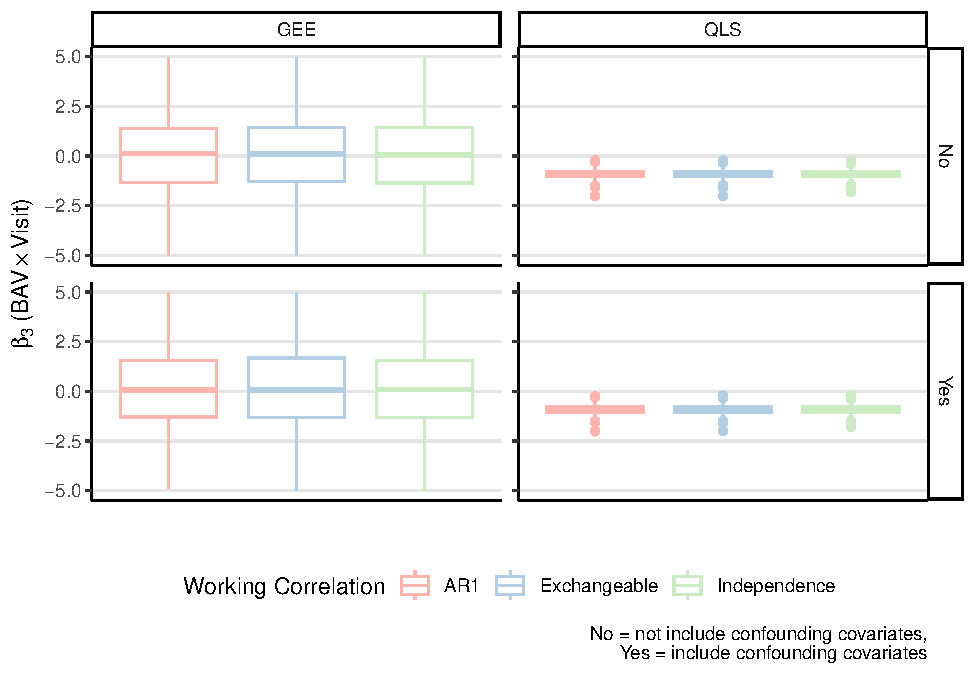
\includegraphics{FinalReport_files/figure-pdf/unnamed-chunk-5-1.pdf}

}

\caption{Comparison of Estimation Results From 1000 Simulation}

\end{figure}%

Table 3 compares the mean estimation of the correlation among
longitudinal measurements using GEE and QLS methods, both adjusted and
unadjusted for age, sex, and BSA. Without adjusting for confounding
covariates, the mean estimate of the correlation using GEE approach with
AR1 working correlation is 0.196 with a relative bias of -0.345, while
QLS provides a closer estimate (0.247) with a smaller relative bias of
-0.176. For the exchangeable correlation, GEE's mean estimate is highly
biased, while QLS remains robust. Adjusting for confounders improves the
estimates for both methods under AR1, with QLS showing more accurate and
less biased estimates with lower MSE. However, when the working
correlation is misspecified as exchangeable, both methods yield biased
estimates.

\begin{table}[!h]
\centering\centering
\caption{\footnotesize Comparison of mean estimation for the correlation among longitudinal measurements using GEE and QLS methods, with and without adjustment for age, sex, and BSA.}
\centering
\resizebox{\ifdim\width>\linewidth\linewidth\else\width\fi}{!}{
\fontsize{8}{10}\selectfont
\begin{tabular}[t]{>{}lllrrrrrr}
\toprule
 & Correlation & Marginal Model & True Value & rho Estimate & SD & Bias & Relative Bias & MSE\\
\midrule
 &  & GEE & 0.3 & 0.196 & 0.161 & -0.104 & -0.345 & 0.036\\
\cmidrule{3-9}
 & \multirow[t]{-2}{*}{\raggedright\arraybackslash AR1} & QLS & 0.3 & 0.247 & 0.196 & -0.053 & -0.176 & 0.041\\
\cmidrule{2-9}
 &  & GEE & 0.3 & 0.095 & 0.118 & -0.205 & -0.685 & 0.056\\
\cmidrule{3-9}
\multirow[t]{-4}{*}[1\dimexpr\aboverulesep+\belowrulesep+\cmidrulewidth]{\raggedright\arraybackslash \textbf{Unadjusted}} & \multirow[t]{-2}{*}{\raggedright\arraybackslash Exchangeable} & QLS & 0.3 & 0.247 & 0.196 & -0.053 & -0.176 & 0.041\\
\cmidrule{1-9}
 &  & GEE & 0.3 & 0.246 & 0.161 & -0.054 & -0.182 & 0.029\\
\cmidrule{3-9}
 & \multirow[t]{-2}{*}{\raggedright\arraybackslash AR1} & QLS & 0.3 & 0.271 & 0.193 & -0.029 & -0.098 & 0.038\\
\cmidrule{2-9}
 &  & GEE & 0.3 & 0.130 & 0.119 & -0.170 & -0.568 & 0.043\\
\cmidrule{3-9}
\multirow[t]{-4}{*}[1\dimexpr\aboverulesep+\belowrulesep+\cmidrulewidth]{\raggedright\arraybackslash \textbf{Adjusted}} & \multirow[t]{-2}{*}{\raggedright\arraybackslash Exchangeable} & QLS & 0.3 & 0.123 & 0.103 & -0.177 & -0.590 & 0.042\\
\bottomrule
\multicolumn{9}{l}{\rule{0pt}{1em}\textsuperscript{*} Adjustments were made during the model fitting by include or exclude age, sex, and BSA}\\
\end{tabular}}
\end{table}

Table 3 displays the mean estimation for model fits with adjustment for
confounding variables.

\section{Discusssion}\label{discusssion}

\subsection{Code chunk}\label{sec-chunks}

But you can set \texttt{echo} option to \texttt{true} locally in the
chunk

\subsection{Text color}\label{sec-summary}

Our format makes applying color on inline text possible using the
\texttt{{[}content{]}\{color=\textless{}name\textgreater{}\}} syntax.
Let's see an example.

Here we are using a special feature of our format which is the coloring
because \textcolor{mypink}{pink is a \textbf{nice} color}.

This is possible thanks to the Lua Filter included in the custom
extension format.


  \bibliography{bibliography.bib}



\end{document}
